\section{Struttura dei Package}
I package principali, figli del root package \textit{it.azraelsec}, che fanno parte del progetto sono i seguenti:
\begin{itemize}
	\item \texttt{Chat} - Cassi che interessate nella gestione del servizio di messaggistica multicast UDP
	\item \texttt{Client} - Classi costituenti il client del sistema TURING
	\item \texttt{Document} - Classi relativi alla rappresentazione dei documenti e delle sezioni costituenti\footnote{I Documenti, infatti, sono formati in realtà da un'aggreazione di differenti Sezioni}
	\item \texttt{Notification} - Classi per la gestione delle notifiche lato client e per la loro generazione lato server
	\item \texttt{Protocol} - Classi ed interfacce atte alla gestione del protocollo di rete \textit{low-level}
	\item \texttt{Server} - Classi costituenti il server del sistema TURING, relative alla gestione del concetto di \textit{Utente} ed al ciclo di vita delle sue sessioni
\end{itemize}
\begin{figure}[h]
	\caption{UML - Package Diagram}
	\centering
	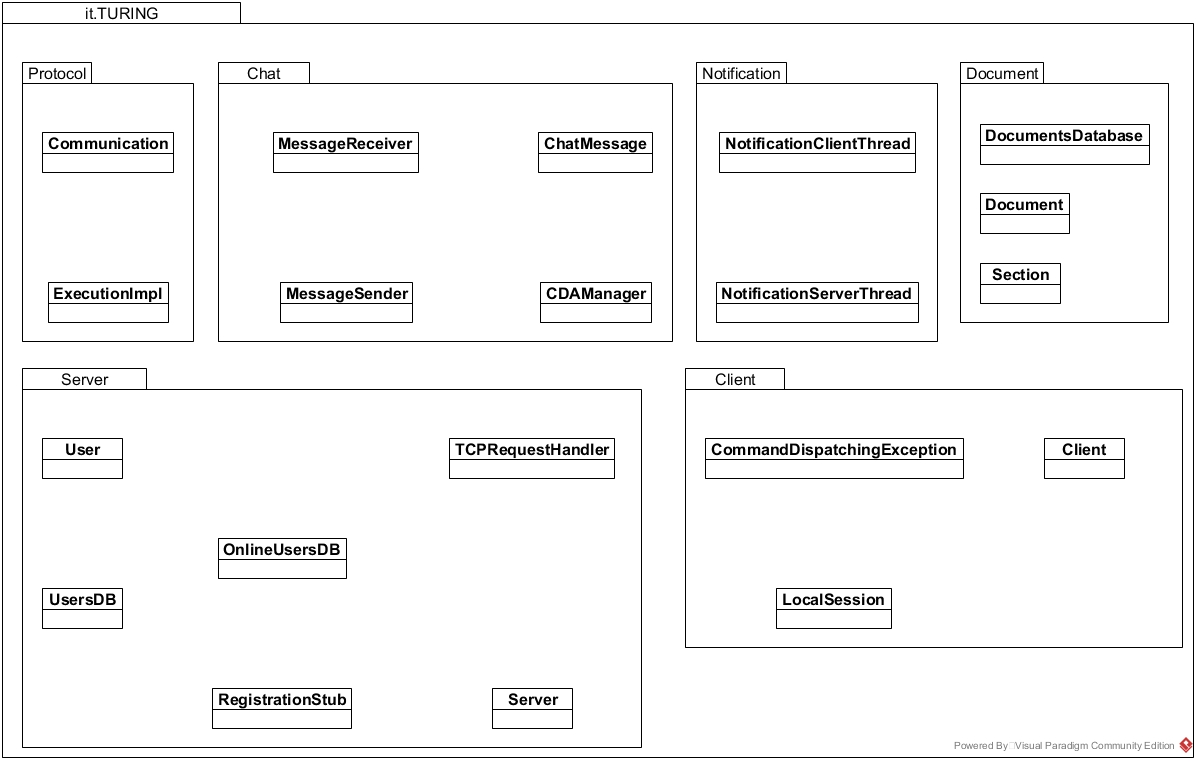
\includegraphics[width=1\linewidth]{assets/package_diagram}
\end{figure}

\pagebreak
